\section{Geometric Mechanics and Control} \label{section:geometric_mechanics}

Geometric control for quadrotor UAVs is first introduced by T. Lee et al. 2010. \cite{LeeClanak4} by presenting a trajectory tracking controller on the SE(3) configuration manifold. Underlying implementation is a proportional-derivative controller with additional nonlinear terms used to cancel the unfavorable dynamics which present themselves during the Lyapunov stability analysis. Starting point for the geometric controller synthesis is the rotating rigid body Lagrangian dynamics equations as follows:
\begin{gather}
m \ddot{\textbf{x}} + m g\textbf{e}_3 = f\text{R}\textbf{e}_3 \label{model1} \\
\text{J}\dot{\mb{\Omega}} + \mb{\Omega} \times \text{J}\mb{\Omega} = \textbf{M} \label{model2} \\
\dot{\text{R}} = \text{R}\reallywidehat{\mb{\Omega}} \label{model3}
\end{gather}
\noindent \textit{Hat map} and \textit{vee map} operators are defined as:
\begin{gather}
\reallywidehat{ \boldsymbol{\cdot} }: \; \mathbb{R}^3 \mapsto \mathfrak{so}(3), \label{eqn:hat} \\
{ \boldsymbol{\cdot} }^\vee: \; \mathfrak{so}(3) \mapsto \mathbb{R}^3 \label{eqn:vee}
\end{gather}
respectively. \\
\noindent It should be pointed out that the notation used for the Special Orthogonal Lie group is SO(3), while its corresponding Lie algebra is denoted by $\mathfrak{so}$(3).

\noindent The following terms are defined as:

\begin{itemize}
	\item $\text{J} \in \mathbb{R}^{3 \times 3}$ - Moment of inertia matrix w.r.t. the body-fixed frame
	
	\item $\text{R} \in \text{SO}(3)$ - Rotation matrix from the body fixed frame to the inertial frame
	
	\item $\mb{\Omega} \in \mathbb{R}^3$ - Angular velocity in the body-fixed frame
	
	\item $\textbf{x} \in \mathbb{R}^3$ - Location of the body-fixed frame in the inertial frame
	
	\item $\textbf{v} \in \mathbb{R}^3$ - Velocity of the body-fixed frame in the inertial frame
	
	\item $f \in \mathbb{R}$ - Total thrust produced by the UAV
	
	\item $\textbf{M} \in \mathbb{R}^3$ - Total moments acting in the body-fixed frame
\end{itemize}

\noindent Utilizing the Lyapunov stability analysis of SE(3) configuration errors appropriate control terms for force $f$ and moments \textbf{M} are derived. In order to translate control force and moments to rotational velocities $\omega_i$ the following relations are employed.
\begin{gather}
f_i = b_f \omega_{i}^2 \label{force}\\
\tau_i = (-1)^i b_m f_i \, ,
\end{gather}
\noindent where the following terms are defined as:	
\begin{itemize}
	\item $f_i \in \mathbb{R}$ - Thrust of the i-th motor
	
	\item $\tau_i \in \mathbb{R}$ - Moment i-th motor produces
	
	\item $b_f \in \mathbb{R}$ - Motor thrust constant
	
	\item $b_m \in \mathbb{R}$ - Motor moment constant
	
	\item $\omega_i \in \mathbb{R}$ - Rotation velocity of the i-th rotor
\end{itemize}
Total thrust can therefore be expressed as:
\begin{equation}
f = \sum_{1}^{4}f_i \, , \label{control:f}
\end{equation}

\noindent Rotor velocities $\omega_i$ and system control inputs ($f$, \textbf{M}) are related using the well known control allocation matrix for cross configuration quadrotors.
\begin{equation}
       \begin{bmatrix}
               f \\
               M_x \\
               M_y \\
               M_z
       \end{bmatrix} = 
       \begin{bmatrix}
               b_f     &       b_f     &       b_f     &       b_f     \\
               0       &       b_f l   &       0       & -b_f l \\
               -b_f l  &       0       &       b_f l   &       0       \\
               b_m b_f &       -b_m b_f        & b_m b_f       & -b_m b_f
       \end{bmatrix} \,
       \begin{bmatrix}
               \omega_1 \\
               \omega_2 \\
               \omega_3 \\
               \omega_4
       \end{bmatrix} \, ,
\end{equation}
\noindent Similar control allocation matrices can be derived for other multirotor UAV configurations.

Another trajectory tracking controller is presented by T. Lee et al. 2011. \cite{LeeClanak3}. Although similar to the original implementation, this controller introduces a quadrotor model with bounded uncertainties in model dynamics, specifically in Eqn. \ref{model1} and \ref{model2}. It can be shown that despite the introduced uncertainties the synthesized tracking controller is robust and the errors are uniformly bounded. The bound can be arbitrarily reduced by control system parameters. 

In \cite{LeeClanak1} and \cite{manuvresGeometric} the default concept of a geometric controller is tested against complex trajectories, such as recovering from an upside down initial position. The controller proved versatile and exhibited almost global asymptotic stability. 

An adaptive geometric controller based on the L1 adaption control law is presented in \cite{Kotaru2019GeometricLA}. A model reference adaptive approach is implemented, with the attitude errors between the quadrotor model and the reference model defined on the manifold. Control laws for the quadrotor and reference models are developed directly on SO(3) to track the desired trajectory while rejecting the uncertainties. Control Lyapunov function based analysis is used to show the exponential input-to-state stability of the attitude errors.

Generally, in the geometric controller, two attitude gains must be provided appropriately to achieve stable error dynamics. The authors in \cite{Lee2019} presented a solution to optimize the controller performance. An Asynchronous Advantage Actor-Critic (A3C) reinforcement learning approach is applied in order to reduce the effort of manual trial-and-error tuning methods. 

The research presented so far considered the quadrotor UAV to be in plus configuration (body-fixed frame aligned with UAV arms) and the center of gravity (CoG) coinciding with the UAV body. However, a novel UAV configuration with dynamic CoG first presented in \cite{movingMass1} and \cite{movingMass2} with initial attitude control structure considered in \cite{movingMass3}. Geometric controller was first implemented for such case in \cite{Markovic2019} using moving masses and a manipulator carrying payload to achieve variations in CoG. A different model is proposed to accommodate changes in CoG and control terms were chosen to achieve exponential stability using Lyapunov functions.
\begin{figure}[H]
	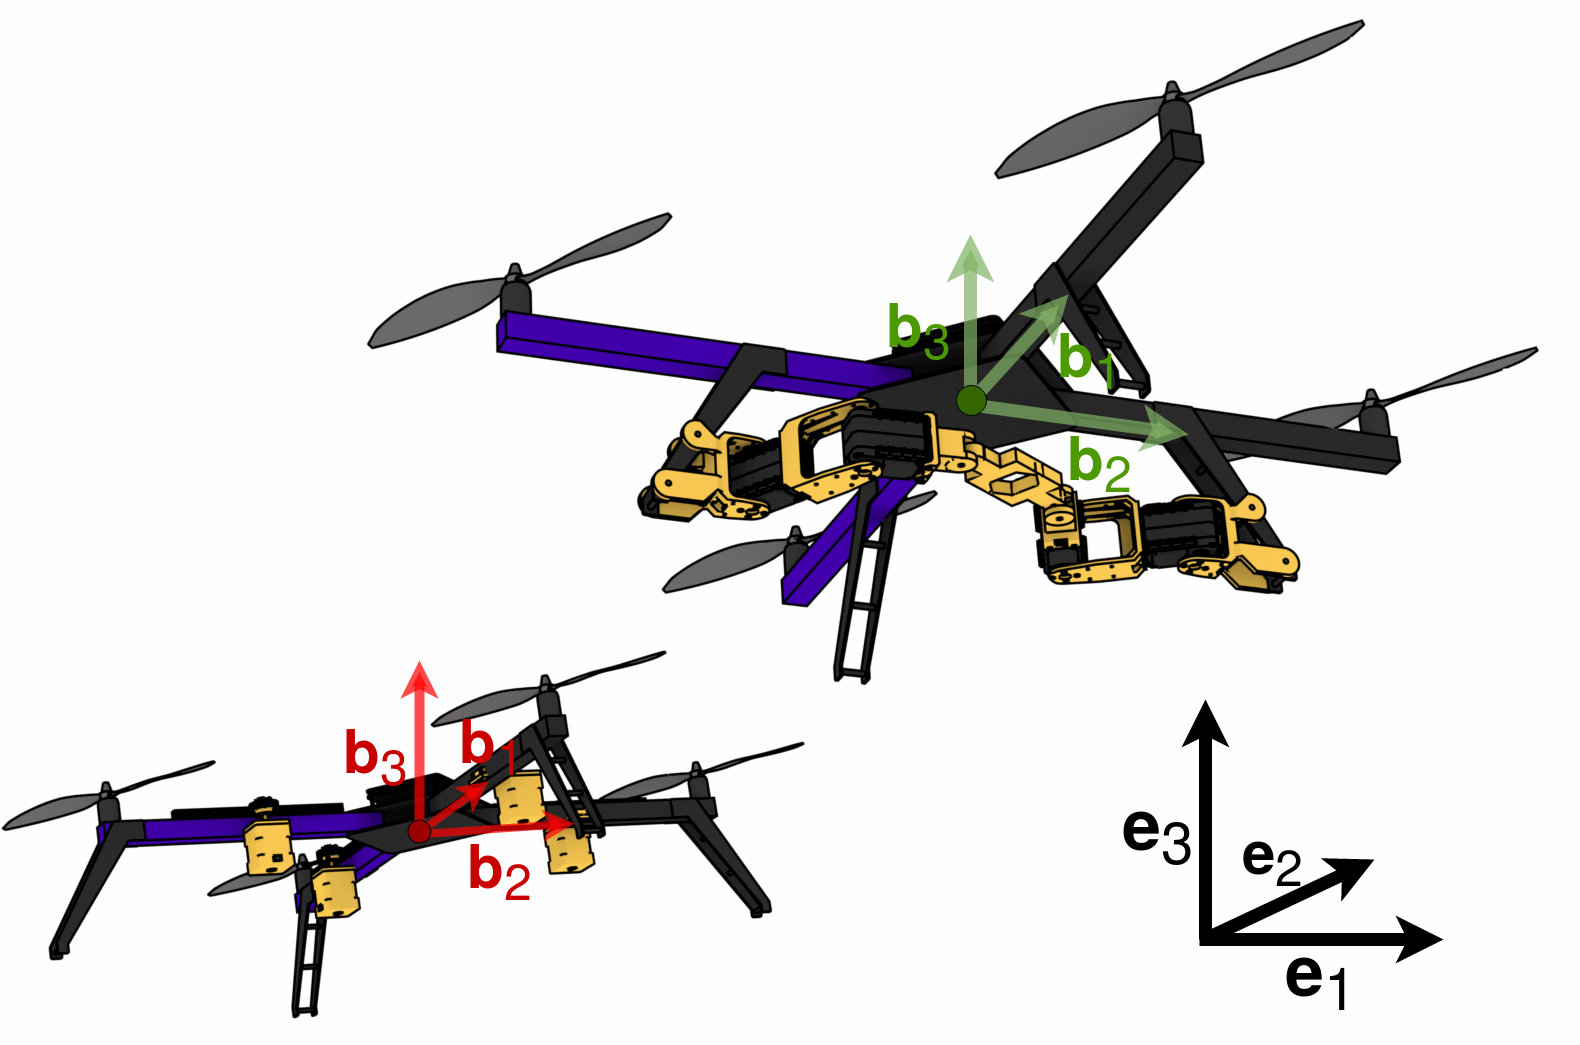
\includegraphics[width=0.8\columnwidth]{figure/uav.png}	
	\centering
	\caption{The $\text{figure}^{\cite{Markovic2019}}$ shows two UAVs endowed with variable moving masses (left) and manipulator carried payload (right). Both UAV concepts are able to offset their center of gravity outside the origin of their body-fixed frame $\{\textbf{b}_1, \textbf{b}_2, \textbf{b}_3\}$. The inertial frame is depicted as $\{\textbf{e}_1, \textbf{e}_2, \textbf{e}_3\}$.  }
	\label{fig:uav_model}
\end{figure}

Another widespread application of the geometric controller are payload transportation tasks. Originally introduced by T. Lee and V. Kumar 2013. \cite{cable-load1}, variations of the concept with multiple quadrotors carrying a payload was presented in \cite{cable-load-multiple} and \cite{Lee2014GeometricCO}. Quadrotor with a flexible cable model and attached load was presented in \cite{tethered-quadrotor}, \cite{flexible-cable}, \cite{flexible-cable-dynamics} and \cite{stabilization-flexible-cable}. Adaptive control along with unknown mass variations are presented in  \cite{rigid-body-transport} and \cite{unknown-mass-transport} respectively.
The overarching idea between all the mention papers considers an underactuated coordinate-free dynamic model of a quadrotor with a cable-suspended load defined on the configuration manifold SE(3)$\times\text{S}^2$, where $\text{S}^2 = \{\textbf{x} \in \mathbb{R}^{3} \,:\, \lVert \textbf{x} \rVert = r \}$. Coordinate-free approach is once again utilized to avoid singularities and complexities that are associated with local parameterizations. A nonlinear geometric control design is developed, that enables tracking of outputs defined by quadrotor and load attitude as well as position of the load. 

\begin{figure}[H]
	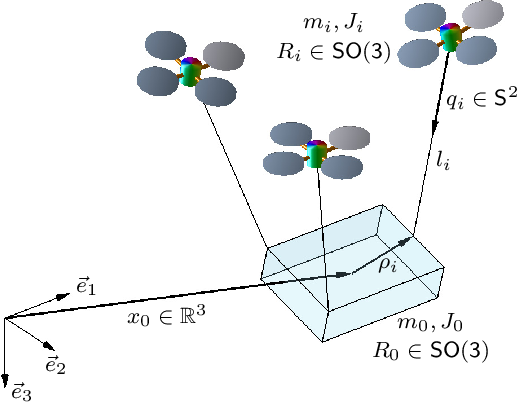
\includegraphics[width=\columnwidth]{figure/payload_carrying.png}	
	\centering
	\caption{This $\text{figure}^{\cite{Lee2014GeometricCO}}$ represents multiple quadrotor UAVs carrying a single rigid-body load via cables. Cable are defined in $\text{S}^2$ - spherical configuration while the UAV remains in SE(3). The underlying coupled system mechanics, therefore, evolve on an SE(3)$\times\text{S}^2$ configuration manifold. }
	\label{fig:load_carrying}
\end{figure}

